%%%%%%%%%%%%%%%%%%%%%%%%%%%%%%%%%%%%%%%%%
% Cleese Assignment (For Students)
% LaTeX Template
% Version 2.0 (27/5/2018)
%
% This template originates from:
% http://www.LaTeXTemplates.com
%
% Author:
% Vel (vel@LaTeXTemplates.com)
%
% License:
% CC BY-NC-SA 3.0 (http://creativecommons.org/licenses/by-nc-sa/3.0/)
% 
%%%%%%%%%%%%%%%%%%%%%%%%%%%%%%%%%%%%%%%%%

%----------------------------------------------------------------------------------------
%	PACKAGES AND OTHER DOCUMENT CONFIGURATIONS
%----------------------------------------------------------------------------------------

\documentclass[11pt]{article}

%%%%%%%%%%%%%%%%%%%%%%%%%%%%%%%%%%%%%%%%%
% Cleese Assignment
% Structure Specification File
% Version 1.0 (27/5/2018)
%
% This template originates from:
% http://www.LaTeXTemplates.com
%
% Author:
% Vel (vel@LaTeXTemplates.com)
%
% License:
% CC BY-NC-SA 3.0 (http://creativecommons.org/licenses/by-nc-sa/3.0/)
% 
%%%%%%%%%%%%%%%%%%%%%%%%%%%%%%%%%%%%%%%%%

%----------------------------------------------------------------------------------------
%	PACKAGES AND OTHER DOCUMENT CONFIGURATIONS
%----------------------------------------------------------------------------------------
\usepackage{lastpage} % Required to determine the last page number for the footer

\usepackage{graphicx} % Required to insert images

\setlength\parindent{0pt} % Removes all indentation from paragraphs

\usepackage[most]{tcolorbox} % Required for boxes that split across pages

\usepackage{booktabs} % Required for better horizontal rules in tables

\usepackage{listings} % Required for insertion of code

\usepackage{etoolbox} % Required for if statements

\usepackage[T1]{fontenc} % Output font encoding for international characters

\usepackage[utf8]{inputenc} % Required for inputting international characters

\usepackage{algorithm}

\usepackage{algpseudocode}
\usepackage{enumitem}
\usepackage{url}
\usepackage{hyperref}



%----------------------------------------------------------------------------------------
%	MARGINS
%----------------------------------------------------------------------------------------

\usepackage{geometry} % Required for adjusting page dimensions and margins

\geometry{
	paper=a4paper, % Change to letterpaper for US letter
	top=3cm, % Top margin
	bottom=3cm, % Bottom margin
	left=2cm, % Left margin
	right=2cm, % Right margin
	headheight=14pt, % Header height
	footskip=1.4cm, % Space from the bottom margin to the baseline of the footer
	headsep=1.2cm, % Space from the top margin to the baseline of the header
	%showframe, % Uncomment to show how the type block is set on the page
}

%----------------------------------------------------------------------------------------
%	FONT
%----------------------------------------------------------------------------------------

\usepackage[utf8]{inputenc} % Required for inputting international characters
\usepackage[T1]{fontenc} % Output font encoding for international characters

\usepackage[sfdefault,light]{roboto} % Use the Roboto font
\fontsize{11pt}{12pt}

%----------------------------------------------------------------------------------------
%	HEADERS AND FOOTERS
%----------------------------------------------------------------------------------------

\usepackage{fancyhdr} % Required for customising headers and footers

\pagestyle{fancy} % Enable custom headers and footers

\lhead{\small\assignmentTitle\ } % Left header; output the instructor in brackets if one was set
\chead{\small\assignmentClass} % Centre header
\rhead{\small\ifdef{\assignmentAuthorName}{\assignmentAuthorName}{\ifdef{\assignmentDueDate}{Due\ \assignmentDueDate}{}}} % Right header; output the author name if one was set, otherwise the due date if that was set

\lfoot{} % Left footer
\cfoot{\small Page\ \thepage\ of\ \pageref{LastPage}} % Centre footer
\rfoot{} % Right footer

\renewcommand\headrulewidth{0.5pt} % Thickness of the header rule

%----------------------------------------------------------------------------------------
%	MODIFY SECTION STYLES
%----------------------------------------------------------------------------------------

\usepackage{titlesec} % Required for modifying sections

%------------------------------------------------
% Section

\titleformat
{\section} % Section type being modified
[block] % Shape type, can be: hang, block, display, runin, leftmargin, rightmargin, drop, wrap, frame
{\Large\bfseries} % Format of the whole section
{\thesection} % Format of the section label
{6pt} % Space between the title and label
{} % Code before the label

\titlespacing{\section}{0pt}{0.5\baselineskip}{0.5\baselineskip} % Spacing around section titles, the order is: left, before and after

% %------------------------------------------------
% % Subsection

% \titleformat
% {\subsection} % Section type being modified
% [block] % Shape type, can be: hang, block, display, runin, leftmargin, rightmargin, drop, wrap, frame
% {\itshape} % Format of the whole section
% {(\alph{subsection})} % Format of the section label
% {4pt} % Space between the title and label
% {} % Code before the label

% \titlespacing{\subsection}{0pt}{0.5\baselineskip}{0.5\baselineskip} % Spacing around section titles, the order is: left, before and after

% \renewcommand\thesubsection{(\alph{subsection})}

%----------------------------------------------------------------------------------------
%	CUSTOM QUESTION COMMANDS/ENVIRONMENTS
%----------------------------------------------------------------------------------------

% Environment to be used for each question in the assignment
\newenvironment{question}{
	\vspace{0.5\baselineskip} % Whitespace before the question
	\section{} % Blank section title (e.g. just Question 2)
	\lfoot{\small\itshape\assignmentQuestionName~\thesection~continued on next page\ldots} % Set the left footer to state the question continues on the next page, this is reset to nothing if it doesn't (below)
}{
	\lfoot{} % Reset the left footer to nothing if the current question does not continue on the next page
}

%------------------------------------------------

% Environment for subquestions, takes 1 argument - the name of the section
\newenvironment{subquestion}[1]{
	\subsection{#1}
}{
}

%------------------------------------------------

% Command to print a question sentence
\newcommand{\questiontext}[1]{
	\textbf{#1}
	\vspace{0.5\baselineskip} % Whitespace afterwards
}

%------------------------------------------------

% Command to print a box that breaks across pages with the question answer
\newcommand{\answer}[1]{
	\begin{tcolorbox}[breakable, enhanced]
		#1
	\end{tcolorbox}
}

%------------------------------------------------

% Command to print a box that breaks across pages with the space for a student to answer
\newcommand{\answerbox}[1]{
	\begin{tcolorbox}[breakable, enhanced]
		\vphantom{L}\vspace{\numexpr #1-1\relax\baselineskip} % \vphantom{L} to provide a typesetting strut with a height for the line, \numexpr to subtract user input by 1 to make it 0-based as this command is
	\end{tcolorbox}
}

%------------------------------------------------

% Command to print an assignment section title to split an assignment into major parts
\newcommand{\assignmentSection}[1]{
	{
			\centering % Centre the section title
			\vspace{1\baselineskip} % Whitespace before the entire section title

			\rule{\textwidth}{0.5pt} % Horizontal rule

			\vspace{0.75\baselineskip} % Whitespace before the section title
			{\LARGE \MakeUppercase{#1}} % Section title, forced to be uppercase

			\rule{\textwidth}{0.5pt} % Horizontal rule

			\vspace{\baselineskip} % Whitespace after the entire section title
			\setcounter{section}{0}
		}
}

%----------------------------------------------------------------------------------------
%	TITLE PAGE
%----------------------------------------------------------------------------------------


\author{\textbf{\assignmentAuthorName}} % Set the default title page author field
\date{} % Don't use the default title page date field

\title{
	\textsc{\LARGE HES-SO Master}\\[1.5cm] % logo Ecole
	
\includegraphics[scale=.2]{images/mse.png}\\[1cm] % Include a department/university logo - this will require the graphicx package
	\thispagestyle{empty} % Suppress headers and footers
	\vspace{0.1\textheight} % Whitespace before the title
	\textbf{\assignmentTitle}\\[4pt]
	\ifdef{\assignmentDueDate}{{\assignmentDueDate}\\}{} % If a due date is supplied, output it
	\ifdef{\assignmentClassInstructor}{{\large \textit{\assignmentClassInstructor}}}{} % If an instructor is supplied, output it
	\vspace{0.32\textheight} % Whitespace before the author name
}
 % Include the file specifying the document structure and custom commands

\renewcommand{\listalgorithmname}{Liste des algorithmes}
\floatname{algorithm}{Algorithme}
\renewcommand{\algorithmicreturn}{\textbf{retourne}}
\renewcommand{\algorithmicprocedure}{\textbf{procédure}}
\renewcommand{\And}{\textbf{et}\ }
\renewcommand{\algorithmicrequire}{\textbf{Entrée:}}
\renewcommand{\algorithmicensure}{\textbf{Sortie:}}
\renewcommand{\algorithmicend}{\textbf{fin}}
\renewcommand{\algorithmicif}{\textbf{si}}
\renewcommand{\algorithmicthen}{\textbf{alors}}
\renewcommand{\algorithmicelse}{\textbf{sinon}}
\renewcommand{\algorithmicfor}{\textbf{pour}}
\renewcommand{\algorithmicforall}{\textbf{pour tout}}
\renewcommand{\algorithmicdo}{\textbf{faire}}
\renewcommand{\algorithmicwhile}{\textbf{tant que}}
\newcommand{\algorithmicelsif}{\algorithmicelse\ \algorithmicif}
\newcommand{\algorithmicendif}{\algorithmicend\ \algorithmicif}
\newcommand{\algorithmicendfor}{\algorithmicend\ \algorithmicfor}
%\renewcommand{\Comment}[1]{\{#1\}}
\renewcommand{\Comment}[1]{\raggedright\hfill\small//~#1}

%----------------------------------------------------------------------------------------
%	ASSIGNMENT INFORMATION
%----------------------------------------------------------------------------------------

% Required
\newcommand{\assignmentQuestionName}{Question} % The word to be used as a prefix to question numbers; example alternatives: Problem, Exercise
\newcommand{\assignmentClass}{IoT} % Course/class
\newcommand{\assignmentTitle}{EthiScan - L'App pour les Consomm'acteurs} % Assignment title or name
\newcommand{\assignmentAuthorName}{Olivier D'Ancona, Clarisse Fleurimont, Yannis Chamot} % Student name

% Optional (comment lines to remove)
\newcommand{\assignmentClassInstructor}{Professeur: Pascal Bruegger \& Aïcha Rizzotti} % Intructor name/time/description
\newcommand{\assignmentDueDate}{Vendredi,\ 14\ Mai\, 2024} % Due date

%----------------------------------------------------------------------------------------

\begin{document}

%----------------------------------------------------------------------------------------
%	TITLE PAGE
%----------------------------------------------------------------------------------------


\clearpage\maketitle % Print the title page
\setcounter{page}{0}
\thispagestyle{empty} % Suppress headers and footers on the title page
\newpage

%----------------------------------------------------------------------------------------
%	TABLE OF CONTENTS
%----------------------------------------------------------------------------------------

\tableofcontents
\newpage

%----------------------------------------------------------------------------------------
%	ABSTRACT
%----------------------------------------------------------------------------------------
\section*{Abstract/Résumé}
\addcontentsline{toc}{section}{Abstract/Résumé}
EthiScan est une application mobile destinée à transformer l'expérience de consommation en permettant aux utilisateurs de scanner des produits pour obtenir des informations détaillées alignées avec leurs valeurs personnelles. Elle vise à promouvoir une consommation responsable en fournissant des données sur les labels environnementaux et nutritionnels, l'évolution des prix, l'impact carbone, et d'autres critères pertinents. En intégrant une technologie de pointe et une conception centrée sur l'utilisateur, EthiScan offre une plateforme fiable et intuitive pour faire des choix de consommation éclairés et responsables.

%----------------------------------------------------------------------------------------
%	INTRODUCTION
%----------------------------------------------------------------------------------------


\section{Introduction}
\subsection{Technologie Utilisée}

EthiScan utilise une stack technologique moderne et efficace pour offrir une expérience utilisateur optimale. Le front-end de l'application est développé avec Flutter, permettant une interface utilisateur cohérente et réactive sur iOS, Android et le Web. Le back-end repose sur Firebase, qui fournit une solution robuste pour l'authentification, le stockage des données, et les fonctionnalités backend nécessaires.

Flutter, avec sa capacité de compilation native, offre des performances élevées et une excellente réactivité, essentielles pour les fonctionnalités de scan en temps réel. L'utilisation de Firebase permet une gestion sécurisée des données utilisateurs et facilite l'intégration d'APIs externes pour la récupération des données produits.

%----------------------------------------------------------------------------------------
%	UX
%----------------------------------------------------------------------------------------


\section{UX}

\subsection{User Stories}

Pour le développement de notre application mobile, nous avons défini plusieurs user stories afin de nous assurer que les besoins des utilisateurs sont pris en compte de manière exhaustive. Voici les user stories que nous avons identifiées :

\subsubsection{User Story 1}

\textbf{En tant qu'utilisat.eur.rice, je veux pouvoir scanner un produit pour obtenir des informations détaillées sur celui-ci.}

\begin{itemize}[noitemsep]
    \item \textbf{Priorité} : Must Have
    \item \textbf{Difficulté} : Moyen
    \item \textbf{Critères d'acceptation} :
          \begin{itemize}[noitemsep]
              \item L'utilisat.eur.rice peut scanner un produit en utilisant la caméra de son téléphone.
              \item L'application affiche les informations détaillées du produit scanné (Metadata).
          \end{itemize}
    \item \textbf{Histoire} : Alice et Bob sont dans un supermarché et veulent acheter des produits alimentaires. Ils veulent pouvoir scanner les produits pour obtenir des informations détaillées sur ceux-ci. Par exemple, ils veulent savoir si le produit est bio, local, s'il contient des allergènes, etc.
\end{itemize}

\subsubsection{User Story 2}

\textbf{En tant qu'utilisat.eur.rice, je veux pouvoir ajouter un produit à une liste de favoris pour un accès rapide.}

\begin{itemize}[noitemsep]
    \item \textbf{Priorité} : Nice to Have
    \item \textbf{Difficulté} : Facile
    \item \textbf{Critères d'acceptation} :
          \begin{itemize}[noitemsep]
              \item L'utilisat.eur.rice peut ajouter un produit à une liste de favoris.
              \item L'utilisat.eur.rice peut consulter sa liste de favoris.
          \end{itemize}
    \item \textbf{Histoire} : Alice et Bob veulent pouvoir ajouter des produits à une liste de favoris pour un accès rapide. Par exemple, ils veulent pouvoir ajouter des produits qu'ils achètent régulièrement à leur liste de favoris.
\end{itemize}

\subsubsection{User Story 3}

\textbf{En tant qu'utilisat.eur.rice, je veux pouvoir configurer mes préférences d'achat pour recevoir des informations personnalisées.}

\begin{itemize}[noitemsep]
    \item \textbf{Priorité} : Must Have
    \item \textbf{Difficulté} : Moyen
    \item \textbf{Critères d'acceptation} :
          \begin{itemize}[noitemsep]
              \item L'utilisat.eur.rice peut configurer ses préférences d'achat (metadata) (local, bio, qualité, prix, impact carbone, durabilité de l'emballage, livrable par la poste).
              \item L'application affiche des informations personnalisées en fonction des préférences de l'utilisat.eur.rice.
          \end{itemize}
    \item \textbf{Histoire} : Alice a scanné un produit et est abonnée au metadata Labels. Elle cherche à trouver le label bio sur le produit scanné.
\end{itemize}

\subsubsection{User Story 4}

\textbf{En tant qu'utilisat.eur.rice, je veux pouvoir consulter les labels et certifications des produits scannés (Certification = Metadata).}

\begin{itemize}[noitemsep]
    \item \textbf{Priorité} : Nice to Have
    \item \textbf{Difficulté} : Moyen
    \item \textbf{Critères d'acceptation} :
          \begin{itemize}[noitemsep]
              \item L'application affiche les labels et certifications des produits scannés.
          \end{itemize}
    \item \textbf{Histoire} : Alice et Bob veulent pouvoir consulter les labels et certifications des produits scannés. Par exemple, ils veulent savoir si le produit est bio, s'il a des labels environnementaux, etc.
\end{itemize}

\subsubsection{User Story 5}

\textbf{En tant qu'utilisat.eur.rice, je veux pouvoir consulter l'évolution du prix des produits scannés (metadata).}

\begin{itemize}[noitemsep]
    \item \textbf{Priorité} : Nice to Have
    \item \textbf{Difficulté} : Moyen
    \item \textbf{Critères d'acceptation} :
          \begin{itemize}[noitemsep]
              \item L'application affiche l'évolution du prix des produits scannés chez différents fournisseurs.
          \end{itemize}
    \item \textbf{Histoire} : Alice et Bob veulent pouvoir consulter l'évolution du prix des produits scannés. Par exemple, ils veulent savoir si le prix du produit a augmenté ou diminué récemment.
\end{itemize}

\subsubsection{User Story 6}

\textbf{En tant qu'utilisat.eur.rice, je veux pouvoir consulter l'impact carbone des produits scannés (metadata).}

\begin{itemize}[noitemsep]
    \item \textbf{Priorité} : Nice to Have
    \item \textbf{Difficulté} : Moyen
    \item \textbf{Critères d'acceptation} :
          \begin{itemize}[noitemsep]
              \item L'application affiche l'impact carbone des produits scannés.
          \end{itemize}
    \item \textbf{Histoire} : Alice et Bob veulent pouvoir consulter l'impact carbone des produits scannés. Par exemple, ils veulent savoir si le produit a un impact carbone élevé ou faible.
\end{itemize}

\subsubsection{User Story 7}

\textbf{En tant qu'utilisat.eur.rice je veux pouvoir avoir accès aux données qui m'intéressent pour pouvoir faire mes choix de produits.}

\begin{itemize}[noitemsep]
    \item \textbf{Priorité} : Must Have
    \item \textbf{Difficulté} : Moyen
    \item \textbf{Histoire} : Alice va faire des courses pour l'anniversaire de Bob. Elle est devant le rayon des gâteaux. Elle scanne un gâteau qui lui fait envie. Elle veut connaître les informations suivantes : présence ou non de cacahuètes, d'où viennent les composants, s'il existe des produits équivalents qui consomment moins de CO2.
\end{itemize}

\subsection{Wireframe}

Après avoir défini les user stories, nous avons créé un wireframe sur Figma pour visualées qui m'intéressent pour pouvoir faire mes choix de produits.}

\begin{itemize}[noitemsep]
    \item \textbf{Priorité} : Must Have
    \item \textbf{Difficulté} : Moyen
    \item \textbf{Histoire} : Alice va faire des courses pour l'anniversaire de Bob. Elle est devant le rayon des gâteaux. Elle scanne un gâteau qui lui fait envie. Elle veut connaître les informations suivantes : présence ou non de cacahuètes, d'où viennent les composants, s'il existe des produits équivalents qui consomment moins de CO2.
\end{itemize}
où viennent les composants, s'il existe des produits équivalents qui consomment moins de CO2.
\end{itemize}

\subsection{Wireframe}

Après avoir défini les user stories, nous avons créé un wireframe sur Figma pour visualiser l'interface utilisateur de notre application et assurer une cohérence visuelle. Ce wireframe a permis de structurer et d'organiser les différents éléments de l'application, tels que les écrans de scan de produit, la configuration des préférences d'achat, et les listes de favoris. En adoptant un style uniforme, nous avons assuré une expérience utilisateur harmonieuse et intuitive. Ce prototype a servi de base pour le développement, facilitant la collaboration entre les concepteurs et les développeurs, et garantissant que tous les aspects fonctionnels et esthétiques de l'application sont alignés avec les attentes des utilisateurs.

\subsection{Design \& Experience}

Dans le cadre du développement de notre application mobile, nous avons utilisé des composants customisés tout en respectant un design strict afin d'assurer une expérience utilisateur optimale. Nous avons défini une palette de couleurs cohérente et attrayante, qui reflète l'identité de notre application et facilite la navigation pour les utilisateurs. Cette palette de couleurs a été appliquée uniformément à travers tous les composants de l'application pour maintenir une cohérence visuelle et renforcer la reconnaissance de la marque.

Tous les composants de l'application, tels que les boutons, les formulaires, les ser l'interface utilisateur de notre application et assurer une cohérence visuelle. Ce wireframe a permis de structurer et d'organiser les différents éléments de l'application, tels que les écrans de scan de produit, la configuration des préférences d'achat, et les listes de favoris. En adoptant un style uniforme, nous avons assuré une expérience utilisateur harmonieuse et intuitive. Ce prototype a servi de base pour le développement, facilitant la collaboration entre les concepteurs et les développeurs, et garantissant que tous les aspects fonctionnels et esthétiques de l'application sont alignés avec les attentes des utilisateurs.

\subsection{Design \& Experience}

Dans le cadre du développement de notre application mobile, nous avons utilisé des composants customisés tout en respectant un design strict afin d'assurer une expérience utilisateur optimale. Nous avons défini une palette de couleurs cohérente et attrayante, qui reflète l'identité de notre application et facilite la navigation pour les utilisateurs. Cette palette de couleurs a été appliquée uniformément à travers tous les composants de l'application pour maintenir une cohérence visuelle et renforcer la reconnaissance de la marque.

Tous les composants de l'application, tels que les boutons, les formulaires, les cartes de produits, et les menus, ont été conçus de manière customisée pour s'adapter à nos besoins spécifiques. Nous avons veillé à ce que chaque composant soit non seulement esthétiquement plaisant mais aussi intuitif et facile à utiliser. Voici quelques-unes des bonnes pratiques en matière d'UX que nous avons implémentées :

\begin{itemize}[noitemsep]
    \item \textbf{Consistance Visuelle} : En utilisant une typographie cohérente et des icônes uniformes, nous avons assuré que l'interface reste claire et organisée, ce qui facilite la navigation pour les utilisateurs.
    \item \textbf{Feedback Immédiat} : Chaque action de l'utilisateur, comme cliquer sur un bouton ou scanner un produit, est accompagnée d'un feedback visuel et/ou sonore immédiat pour confirmer que l'action a été enregistrée et est en cours de traitement.
    \item \textbf{Accessibilité} : Nous avons pris soin d'intégrer des fonctionnalités d'accessibilité telles que des contrastes de couleurs suffisants (pour les daltoniens), des polices de caractères ajustables.

    \item \textbf{Navigation Intuitive} : La structure de navigation a été pensée pour être intuitive, avec un menu en 3 points qui a un certain avantage d'accessibilité.

    \item \textbf{Minimisation de la Charge Cognitive} : En évitant les informations superflues et en présentant les données de manière claire et concise, nous avons réduit la charge cognitive de l'utilisateur, facilitant ainsi la prise de décision rapide et informée.

    \item \textbf{Éléments Tactiles Optimisés} : Les zones tactiles pour les interactions ont été conçues de manière à être suffisamment grandes pour éviter les erreurs de manipulation, et les transitions entre les écrans sont fluides pour offrir une expérience utilisateur agréable, grâce aux push et swap de pages.

    \item \textbf{Simplicité et Clarté} : L'interface a été simplifiée pour que chaque écran ne présente que les informations nécessaires, sans surcharge, afin que les utilisateurs puissent se concentrer sur leur tâche principale sans distractions.

    \item \textbf{Internationalisation} : L'application est disponible en plusieurs langues, ce qui permet aux utilisateurs de choisir la langue qui leur convient le mieux. Le processus est décrit dans la section \ref{sec:i18n}
\end{itemize}

Grâce à l'intégration des bonnes pratiques vu en cours, l'expérience utilisateur est plaisante et agréable.

%----------------------------------------------------------------------------------------
%	EVALUATIONS
%----------------------------------------------------------------------------------------


\section{Évaluations}
\subsection{Évaluations Implémentées}

L'évaluation de l'application s'est concentrée sur la performance, l'exactitude des données, et la satisfaction utilisateur. Des tests de performance ont été réalisés pour s'assurer que l'application répond rapidement aux requêtes de scan. L'exactitude des informations fournies a été vérifiée contre des sources externes pour garantir la fiabilité des données. Enfin, des enquêtes de satisfaction utilisateur ont aidé à recueillir des retours sur l'expérience d'utilisation, permettant d'identifier les domaines d'amélioration.

%----------------------------------------------------------------------------------------
%	TECHNIQUES
%----------------------------------------------------------------------------------------


\section{Développement Technique}

\subsection{Peuplement de la base de données}

Pour peupler la base de données de notre application, nous avons rassemblé des données disponibles librement et publiquement sur Internet, en particulier sur les sites de la Migros, de la Coop et de Denner. Ces sites fournissent des métadonnées des articles, incluant leurs prix et des images associées. Nous avons débuté par la création d'un script en Dart qui intègre les produits, certaines métadonnées, ainsi que quelques types de produits et utilisateurs, afin de tester l'application de manière adéquate. Ce script se connecte à Firestore et envoie les données sur Firebase, ce qui permet de peupler efficacement la base de données. Bien que ce script manuel soit initialement utilisé pour insérer les données nécessaires au test de l'application, nous envisageons à l'avenir de développer un scraper web. Ce scraper pourrait automatiser la récupération des données de tous les produits des sites de la Migros, de la Coop, etc., garantissant ainsi une base de données complète et constamment mise à jour. Grâce à cette automatisation, nous pourrions maintenir une base de données riche et précise, essentielle pour le bon fonctionnement de l'application.

\subsection{Internationalisation}
\label{sec:i18n}

Nous avons localisé notre application avec le mécanisme d'internationalisation (i18n) de Flutter. Concrètement, nous avons créé un fichier utilitaire i18n qui nous permet de gérer les différentes traductions de l'application. Chaque langue est représentée par un fichier de traduction spécifique, dans lequel sont stockées les chaînes de caractères traduites. Le processus de traduction commence par l'identification des chaînes de texte à traduire dans l'application. Ensuite, ces chaînes sont externalisées dans les fichiers de traduction, où chaque langue dispose de ses propres traductions. Grâce à ce système, l'application peut automatiquement afficher le texte dans la langue choisie par l'utilisateur, en fonction des paramètres de son appareil. Bie que nous n'ayons pas eu le temps de traduire toutes les chaînes de texte de l'application, le principe de l'internationalisation est entièrement implémenté et fonctionnel. Ainsi, l'ajout de nouvelles traductions peut se faire rapidement et efficacement à mesure que de nouvelles langues sont prises en charge ou que de nouvelles chaînes de texte sont ajoutées à l'application.

\subsection{Modélisation des Données}
\label{sec:data_model}

La structure de données d'EthiScan, illustrée dans la figure \ref{fig:diagramme_classe} a été conçue pour permettre une gestion efficace et évolutive des informations produits et des préférences utilisateurs.

La classe principale \texttt{EthiscanUser} représente un utilisateur de l'application, incluant ses produits favoris (\texttt{FavoriteProduct}), ses préférences (\texttt{UserPreferences}), et un Firebase \texttt{User} contenant des informations d'authentification comme l'identifiant, le nom et l'email. Chaque \texttt{FavoriteProduct} référence un \texttt{Product} avec une date d'ajout, permettant à l'utilisateur de suivre ses produits préférés.

La classe \texttt{Product} représente les produits scannés par les utilisateurs. Chaque produit peut avoir une certification (\texttt{Certification}) et est associé à une liste de métadonnées spécifiques (\texttt{ProductMetadata}). Cette séparation entre le type de métadonnées (\texttt{MetadataType}) et les instances spécifiques des métadonnées permet une gestion flexible des différentes informations que les utilisateurs peuvent consulter.

Les fournisseurs (\texttt{Supplier}) sont modélisés pour contenir une liste de produits vendus (\texttt{SoldProduct}), chacun ayant un prix spécifique. Cette approche permet de gérer les variations de prix d'un même produit chez différents fournisseurs.

Enfin, les préférences utilisateur (\texttt{UserPreferences}) sont représentées par une liste de types de métadonnées auxquels l'utilisateur est abonné. Ces abonnements permettent à l'utilisateur de recevoir des informations personnalisées et pertinentes en fonction de ses valeurs et de ses préférences de consommation.

\begin{figure}[h]
    \centering
    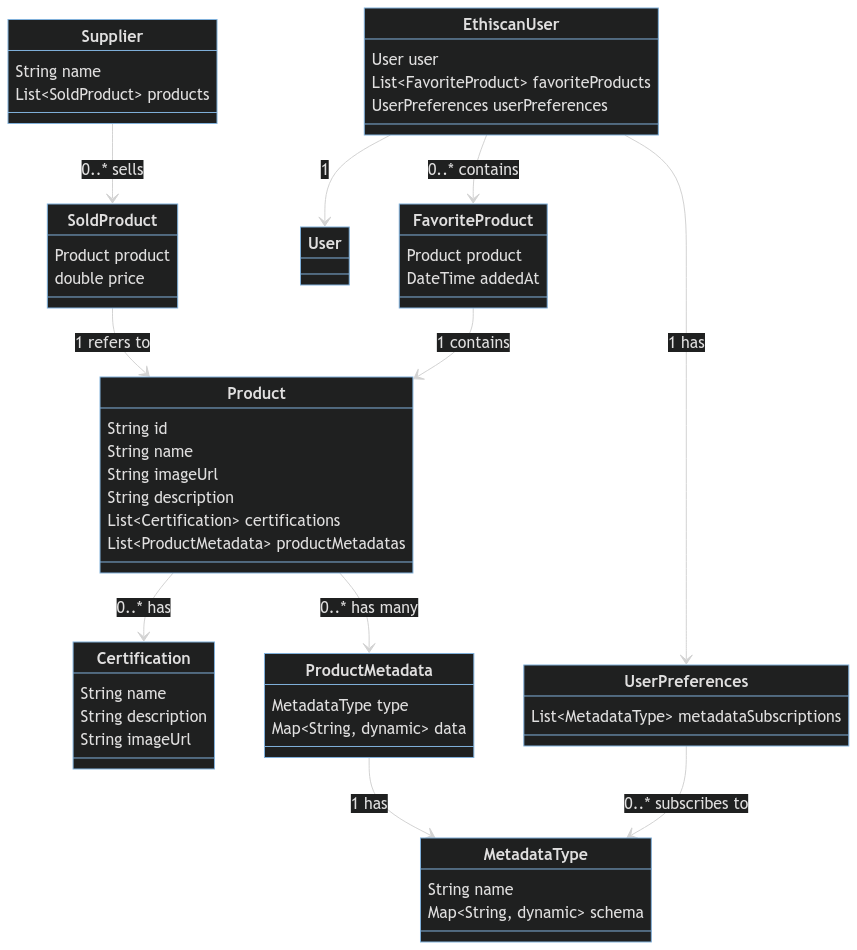
\includegraphics[width=0.6\textwidth]{/home/olivier/projet/advanced_mobile_app/concept/rapport/images/diagramme_classe.png}
    \caption{Diagramme de classe de l'application}
    \label{fig:diagramme_classe}
\end{figure}

\subsection{Intégration Continue et Déploiement Continu (CI/CD)}
\label{sec:ci_cd}
Pour automatiser le processus de développement et de déploiement de notre application mobile, nous avons mis en place des GitHub Actions. Ces workflows permettent de s'assurer que chaque modification apportée au code est correctement testée et que les versions de l'application sont déployées de manière fluide. Nous avons segmenté notre approche CI/CD en deux parties distinctes : l'intégration continue (CI) et le déploiement continu (CD).

\subsubsection{Intégration Continue (CI)}

L'intégration continue est déclenchée à chaque fois qu'un commit est effectué dans le dépôt GitHub. Le but principal de la CI est de garantir la qualité et la cohérence du codebase. Pour ce faire, nous avons configuré GitHub Actions pour exécuter les tests unitaires et le linter sur l'ensemble du code. En particulier, nous utilisons la commande \texttt{flutter analyze} pour analyser notre code Flutter. Cette analyse permet de détecter les erreurs et les incohérences dans le code, facilitant ainsi la collaboration entre les développeurs et assurant que le code est toujours dans un état prêt à être fusionné.

\subsubsection{Déploiement Continu (CD)}

Le déploiement continu est activé à chaque fois qu'un tag est poussé sur le dépôt. Ce processus comprend la construction de l'application et son déploiement. Nous avons configuré une action pour compiler l'application et générer les fichiers APK nécessaires. Une fois la construction terminée, les fichiers APK sont automatiquement envoyés sur notre groupe Telegram. Ceci permet à l'équipe de disposer immédiatement des nouvelles versions de l'application.

\subsection{Problèmes Rencontrés et Solutions}
\label{sec:problems}

\paragraph{Version des dépendances} Lors du développement, nous avons rencontré un problème majeur lié à la gestion des versions de Flutter utilisées par les différents membres de l'équipe. En effet, nous avons constaté qu'une personne utilisait la version 3.22 de Flutter, tandis que d'autres travaillaient avec la version 3.19. Cette disparité de versions a causé des conflits lors de l'intégration de nouvelles dépendances. Par exemple, certaines dépendances étaient compatibles avec une version de Flutter mais pas avec l'autre, ce qui a entraîné des erreurs de compilation. La synchronisation des versions de Flutter entre tous les membres de l'équipe s'est avérée difficile. Nous avions le choix entre downgrade Flutter ou de résoudre les conflits avec la dernière version. Nous avons opté pour la deuxième option, car elle nous permettait de bénéficier des dernières fonctionnalités et correctifs de Flutter. Cependant, cela a nécessité un effort supplémentaire pour résoudre les conflits et garantir la compatibilité des dépendances avec la version la plus récente de Flutter.

\paragraph{Structure de l'application} Nous avons décidé de suivre les bonnes pratiques de la "clean architecture" ce qui a posé plusieurs défis. Comme chaque membre de l'équipe avait une expérience différente Flutter, nous avons tous développé des portions de code de manière indépendante, en utilisant des approches et des structures différentes, souvent inspirées d'exemples trouvés en ligne ou de projets précédents. L'intégration de ces morceaux de code disparates dans un cadre uniforme basé sur la clean architecture a nécessité des efforts significatifs. Nous avons dû refactorer et harmoniser les différentes méthodes de développement pour les aligner avec les principes de la clean architecture, ce qui a parfois causé des problèmes d'intégration et ralenti le développement de nouvelles features. Cette étape a souligné l'importance de définir dès le départ une architecture claire et partagée par toute l'équipe pour faciliter le développement collaboratif. Au final, nous avons utilisé le package "clean\_architecture" pour structurer notre application.

\paragraph{Gestion des états} Un autre défi a été la gestion des blocs, en particulier avec les pages de connexion et d'inscription. Initialement, nous avions un mainUserBloc chargé de l'authentification et de la gestion des données utilisateur dans toute l'application. Cependant, l'intégration des pages de connexion et d'inscription a posé problème. Ces pages, conçues pour fonctionner indépendamment, ne s'intégraient pas bien dans la structure de l'application en raison de problèmes liés aux locales de traduction. Pour contourner ce problème, nous avons décidé de placer ces pages directement dans le fichier app.dart, en dehors de la structure principale de l'application. Cette décision a introduit des complications avec le main user bloc, entraînant des conflits entre les blocs de gestion d'état. Bien que nous ayons finalement trouvé une solution. TODO Quelle solution ? Comment on a fix ce truc ?

\paragraph{Versionnement du code} Nous avons rencontré quelques problèmes avec l'utilisation de GitHub au sein de notre équipe. L'un des membres, ne maîtrisant pas GitHub, a effectué tout son travail sur une branche existante déjà mergée sur la principale (main), sans jamais fusionner ses modifications. Par conséquent, le reste de l'équipe n'a pas pu suivre l'avancement de son travail. Au moment de fusionner sa branche, nous avons découvert le problème. Cela a posé des problèmes d'intégration car le code sur main avait été largement restructuré entre-temps. Pour résoudre cette situation, nous avons résolu les conflits de versions progressivement jusqu'au succès. Puis, nous avons formé toute l'équipe à l'utilisation de GitHub. Désormais, chaque nouvelle tâche doit être accompagnée de la création d'une issue et d'une branche correspondante. Une fois la tâche terminée et approuvée, la branche est fusionnée dans la branche principale avec un code review. Cette approche, combinée à une meilleure communication entre les membres de l'équipe, a permis d'éviter les problèmes.

\paragraph{Déploiement Continu} Le déploiement a posé quelques difficultés, principalement liées à la gestion sécurisée du fichier \texttt{google-service.json}, indispensable pour la construction et le déploiement de l'application sur notre groupe Telegram. Comme ce fichier contient des informations sensibles, nous devons le sécuriser et le stocker dans un endroit accessible par notre pipeline CI/CD. Pour résoudre ce problème, nous avons décidé de stocker \texttt{google-service.json} en tant que action secret dans GitHub. Cependant, un problème de formatage est apparu lors de la gestion de ce secret. Pour le surmonter, nous avons encodé le fichier en base64 avant de le stocker dans GitHub Secrets. Ce qui a résolu le problème de formatage et nous a permis de déployer l'application avec succès de manière sécurisée.

\paragraph{Développement Automatisé}
Pour accélérer le développement, nous avons intégré le package \texttt{Freezed} et encore le package \texttt{json\_encode}, destiné à compiler et générer automatiquement certaines parties du code. Cette automatisation vise à réduire le code répétitif, augmentant ainsi notre productivité et permettant de se concentrer sur des aspects plus critiques du développement. Cependant, l'introduction de ce package a posé des défis pour un membre de l'équipe non familier avec cette technologie. En effet, il rencontrait des difficultés à déboguer son code, n'ayant pas une maîtrise complète des processus automatisés par \texttt{Freezed}. Ce manque de compréhension a entraîné des erreurs de compilation et une perte de temps significative pour cette personne, contrebalançant ainsi les bénéfices attendus de l'automatisation. Pour résoudre ce problème, nous avons organisé une session de discussion afin de clarifier l'utilisation du script \texttt{Freezed} et de bien séparer les concepts. Après cette mise au point, il n'a plus rencontré de problèmes de compilation, et l'équipe a pu bénéficier pleinement des gains de productivité promis par l'automatisation. Cette expérience souligne l'importance de l'accompagnement et de la formation lors de l'intégration de nouvelles technologies dans un projet de développement.


\subsection{Conclusion Technique}

La combinaison de Flutter et Firebase a prouvé son efficacité pour développer une application mobile performante et réactive. L'architecture choisie a permis une mise en œuvre rapide des fonctionnalités tout en maintenant une haute qualité et fiabilité des données.

\section{Auto-Critique du Code}

\subsection{Points Positifs}
\begin{itemize}
    \item Code bien structuré et commenté, facilitant la maintenance et les mises à jour.
    \item Utilisation efficace des patterns de conception pour une architecture solide.
\end{itemize}

\subsection{Points à Améliorer}

Pour améliorer le développement de notre application mobile, nous avons identifié plusieurs aspects nécessitant des améliorations.

\paragraph{Augmentation de la couverture des tests unitaires}
Actuellement, la couverture de code par nos tests unitaires est insuffisante. Les tests unitaires sont très limités et ne couvrent pas l'ensemble des fonctionnalités critiques de l'application. Pour garantir une meilleure qualité et fiabilité du code, il est impératif d'augmenter la couverture des tests unitaires. Cela inclut l'ajout de tests pour les cas limites, les scénarios d'erreur, ainsi que les interactions complexes entre les différents composants de l'application.

\paragraph{Renforcement de la sécurité des données}
Pour des raisons de développement, les règles de sécurité de notre base de données Firestore sont actuellement complètement ouvertes. Cette configuration est inadmissible dans un environnement de production réel. Il est crucial de mettre en place des règles de sécurité strictes afin de gérer correctement les autorisations des utilisateurs. Chaque utilisateur doit uniquement pouvoir accéder et modifier ses propres données. Par exemple, les règles de sécurité doivent garantir qu'un utilisateur ne puisse pas supprimer ou accéder aux produits favoris d'un autre utilisateur. Le renforcement de ces mesures de sécurité est impératif pour la mise en production de l'application.



%----------------------------------------------------------------------------------------
%	ANNEXES
%----------------------------------------------------------------------------------------

\section{Annexes}

\subsection{Planning Actualisé Avant/Après}

Pour notre projet, nous avons opté pour une organisation méthodique en utilisant un tableau Kanban et une répartition des tâches sur GitHub, plutôt que de suivre un planning formel. Le tableau Kanban nous a permis de structurer le travail en plusieurs colonnes : "À faire", "En cours", "À valider" et "Terminé", offrant ainsi une vue d'ensemble claire de l'état d'avancement du projet et facilitant la coordination. Sur GitHub, chaque tâche était associée à une issue, assignée à des membres spécifiques de l'équipe, ce qui a permis un suivi précis des responsabilités et de l'avancement. Cette méthode de travail nous a permis de prioriser les tâches critiques, de tenir des réunions régulières pour synchroniser nos efforts et de rester flexibles face aux imprévus, assurant ainsi une gestion efficace et adaptative du projet, même sans planning détaillé.

\subsection{Liste des Bugs Connus}

\begin{itemize}[noitemsep]
    \item Overflow sur le login
    \item Impossible de lancer la caméra sur Linux ou Chrome
    \item Si un product n'a pas le même id que son docId, il ne peut pas être supprimé
\end{itemize}

\subsection{Dépendances}

\begin{table}[h!]
    \centering
    \begin{tabular}{|m{0.35\textwidth}|m{0.45\textwidth}|}
        \hline
        \textbf{Package}                 & \textbf{Version} \\ \hline
        flutter                          & sdk: flutter     \\ \hline
        injectable                       & \texttt{>2.4.0}  \\ \hline
        flutter\_localizations           & sdk: flutter     \\ \hline
        cupertino\_icons                 & \texttt{>1.0.6}  \\ \hline
        flutter\_clean\_architecture     & \texttt{>5.0.4}  \\ \hline
        firebase\_core                   & \texttt{>2.25.5} \\ \hline
        flutter\_svg                     & \texttt{>2.0.4}  \\ \hline
        syncfusion\_flutter\_charts      & \texttt{>21.2.4} \\ \hline
        shared\_preferences              & \texttt{>2.2.2}  \\ \hline
        jwt\_decoder                     & \texttt{>2.0.1}  \\ \hline
        flutter\_dotenv                  & \texttt{>5.1.0}  \\ \hline
        flutter\_launcher\_icons         & \texttt{>0.13.1} \\ \hline
        flutter\_i18n                    & \texttt{>0.35.1} \\ \hline
        get\_it                          & \texttt{>7.1.3}  \\ \hline
        firebase\_auth                   & \texttt{>4.19.2} \\ \hline
        cloud\_firestore                 & \texttt{>4.17.3} \\ \hline
        provider                         & \texttt{>6.1.2}  \\ \hline
        bloc                             & \texttt{>8.1.2}  \\ \hline
        flutter\_bloc                    & \texttt{>8.1.3}  \\ \hline
        path\_provider                   & \texttt{>2.0.2}  \\ \hline
        auto\_size\_text                 & \texttt{>3.0.0}  \\ \hline
        freezed\_annotation              & \texttt{>2.2.0}  \\ \hline
        camera                           & \texttt{>0.11.0} \\ \hline
        google\_mlkit\_barcode\_scanning & \texttt{>0.12.0} \\ \hline
        http                             & \texttt{>1.2.1}  \\ \hline
        intl                             & \texttt{>0.19.0} \\ \hline
        json\_annotation                 & \texttt{>4.9.0}  \\ \hline
        uuid                             & \texttt{>4.4.0}  \\ \hline
        phone\_number\_controller        & \texttt{>1.0.4}  \\ \hline
    \end{tabular}
    \caption{Dépendances du projet}
    \label{table:dependencies}
\end{table}

\begin{table}[h!]
    \centering
    \begin{tabular}{|m{0.35\textwidth}|m{0.45\textwidth}|}
        \hline
        \textbf{Package}      & \textbf{Version} \\ \hline
        injectable\_generator & \texttt{>2.1.5}  \\ \hline
        build\_runner         & \texttt{>2.0.5}  \\ \hline
        json\_serializable    & \texttt{>6.1.4}  \\ \hline
        freezed               & \texttt{>2.4.7}  \\ \hline
        flutter\_test         & sdk: flutter     \\ \hline
        flutter\_lints        & \texttt{>4.0.0}  \\ \hline
    \end{tabular}
    \caption{Dépendances de développement du projet}
    \label{table:dev-dependencies}
\end{table}


\subsection{Aides Extérieures}

\begin{itemize}[noitemsep]
    \item Documentation officielle de Flutter : \cite{flutterDocs}
    \item Documentation officielle de Firebase: \cite{firebaseDocs}
    \item Documentation de FlutterFire pour l'intégration de Firebase: \cite{flutterFireDocs}
    \item Clean Architecture: \cite{cleanArchitecture}
    \item Figma pour la conception de l'interface utilisateur: \cite{figma}
    \item Design Pattern du Bloc: \cite{blocPattern}
    \item Site de la Migros: \cite{migros}
    \item Site de la Coop: \cite{coop}
    \item Site de Denner: \cite{denner}
    \item Architecture : \cite{googleCloudArchitecture}
    \item Projet existant : un membre du groupe travail sur un projet d'application mobile et le style visuel de l'application a été inspiré de ce projet (couleurs, design, etc.) \url{https://datamama.ch/}
\end{itemize}


\subsection{Wireframe}
\label{doc:wireframe}

\begin{figure}[H]
    \centering
    \includegraphics[width=0.8\textwidth]{images/wireframe.png}
    \caption{Wireframe de l'application}
    \label{doc:wireframe}
\end{figure}

\subsection{Cahier des charges original}

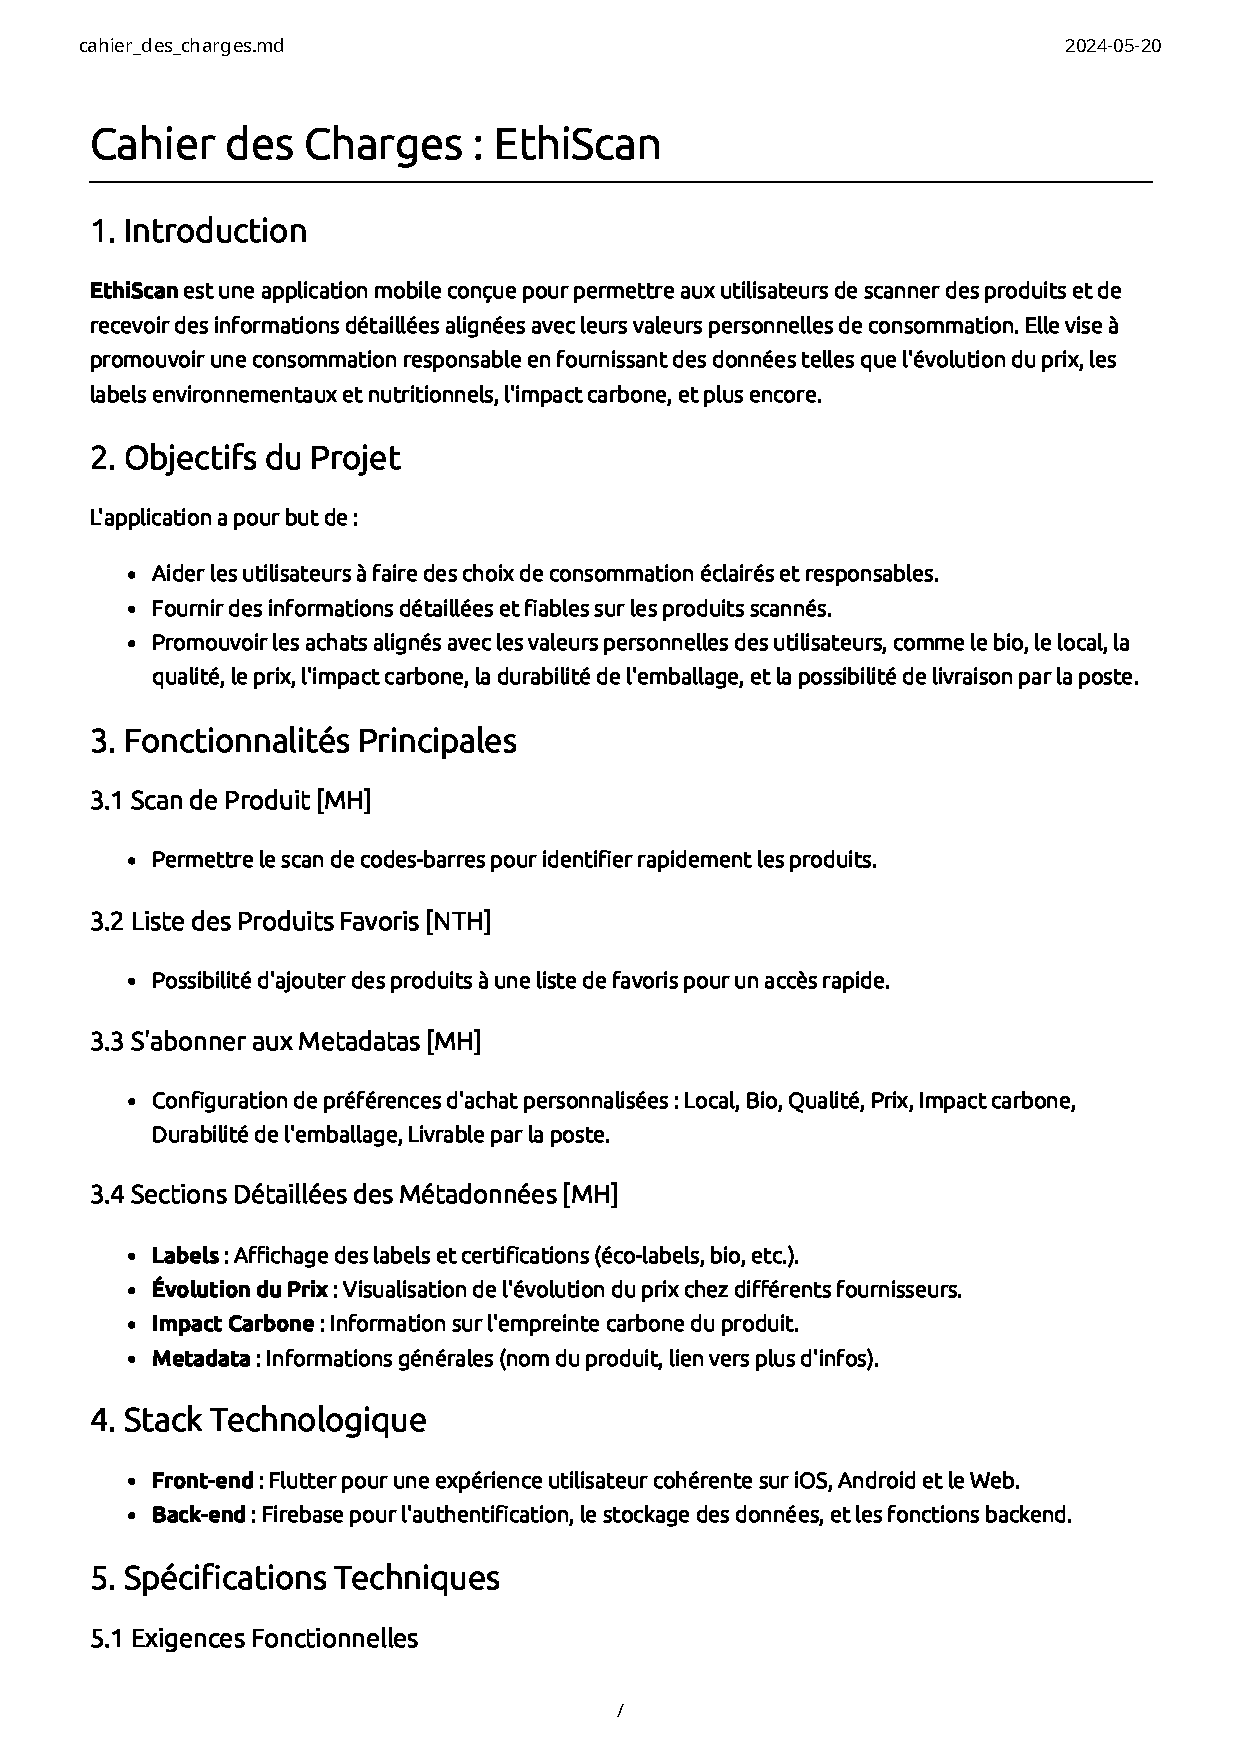
\includepdf[pages=-]{images/cahier_des_charges.pdf}

%----------------------------------------------------------------------------------------
%	BIBLIOGRAPHY
%----------------------------------------------------------------------------------------
\bibliographystyle{plain}
\bibliography{references}


\end{document}
